\subsection{Printed Circuit Board Design} \label{sec:pcb-design}
\noindent It is advantageous to use the 5V configuration for ESP32 UART bridge. In development, we used a development board to program the MCU but in practice must implement a UART bridge on the PCB to communicate with the MCU for flashing the memory and sending serial data out.\\

\noindent For voltage regulation, it could be expedient to, instead of using Texas Instruments Webench to design circuits for the PCB, use a 1/3 voltage divider for the ultrasonic ECHO pins. This is necessary because the ESP32 operates on 3.3V while the ultrasonic sensors use 5V, even though they are 3.3V compatible. This can be easily implemented by a 1k$\Omega$ and 2k$\Omega$ resistor in series.\\

\noindent One other consideration are the PCB traces. We intend to use 20mil (0.5mm) isolations and traces. The PCB does not use RF signals.\\

\noindent Motor controllers are more sensitive components and should be implemented on an independent PCB. These are considered as optically isolated motor drivers in order to minimize back EMI/F. In this case, one would bias an LED to turn the controller on. \cite{l293n}\\

\begin{figure}[H]
	\centering
	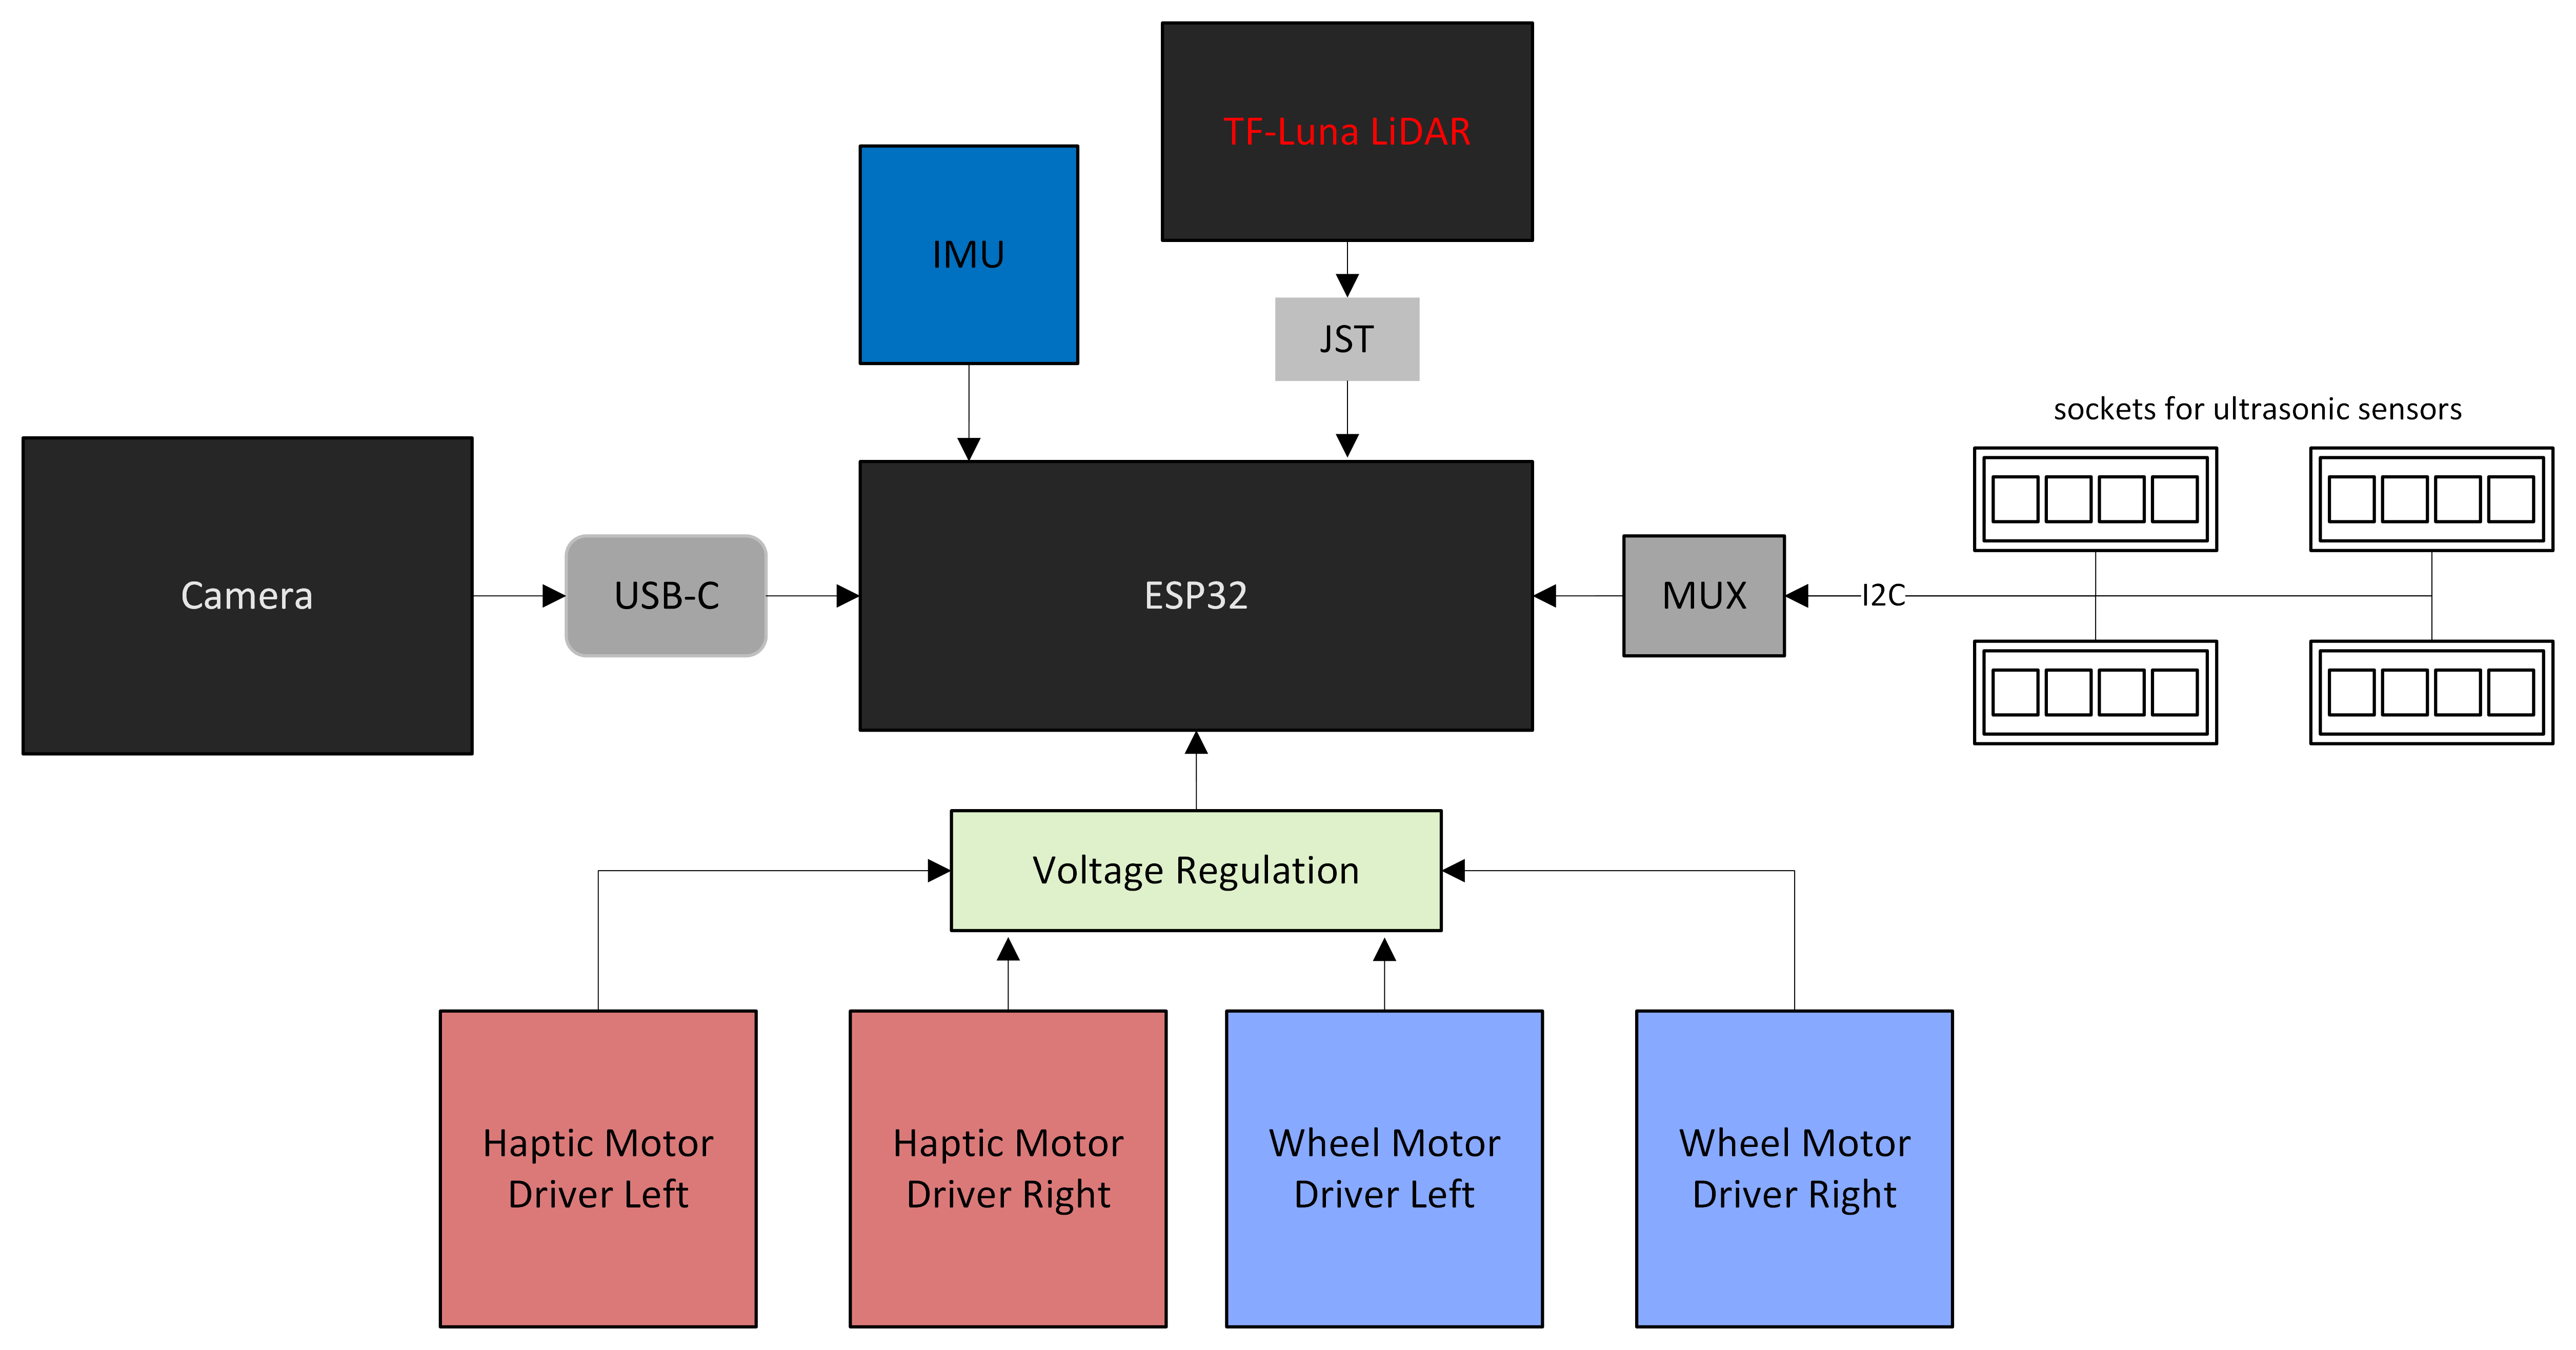
\includegraphics[width=\textwidth]{./Images/PCB-Block-Diagram.png}
	\caption{\label{fig:pcb}PCB Block Diagram}
\end{figure}

\begin{figure}[H]
	\centering
	\includegraphics[width=\textwidth]{./Images/PCB-sch.png}
	\caption{\label{fig:pcb-sch}PCB KiCAD Schematic}
\end{figure}